\documentclass{minimal}
\usepackage{tikz}

% define a sin/cos wave pair of desired frequency illustrating positional encoding in attention transformers
\newcommand{\SinCos}[2]{
    \begin{scope}[xscale=(5/#2)/2]
        \draw[color=#1!60] (-1,0) sin (0,1) cos (1,0) sin (2,-1) cos (3,0) sin (4,1) cos (5,0) sin (6,-1) cos (7,0) sin (8,1) cos (9,0) sin (10,-1) cos (11,0) sin (12,1);
        \draw[color=#1!60!black, xshift=28pt] (-1,0) sin (0,1) cos (1,0) sin (2,-1) cos (3,0) sin (4,1) cos (5,0) sin (6,-1) cos (7,0) sin (8,1) cos (9,0) sin (10,-1) cos (11,0) sin (12,1);

%        absolute value version
%        \draw[color=#1!60] (-1,0) sin (0,1) cos (1,0) sin (2,1) cos (3,0) sin (4,1) cos (5,0) sin (6,1) cos (7,0) sin (8,1) cos (9,0) sin (10,1) cos (11,0) sin (12,1);
%        \draw[color=#1!60!black, xshift=28pt] (-1,0) sin (0,1) cos (1,0) sin (2,1) cos (3,0) sin (4,1) cos (5,0) sin (6,1) cos (7,0) sin (8,1) cos (9,0) sin (10,1) cos (11,0) sin (12,1);
    \end{scope}
}

\begin{document}
    \usetikzlibrary {datavisualization}
    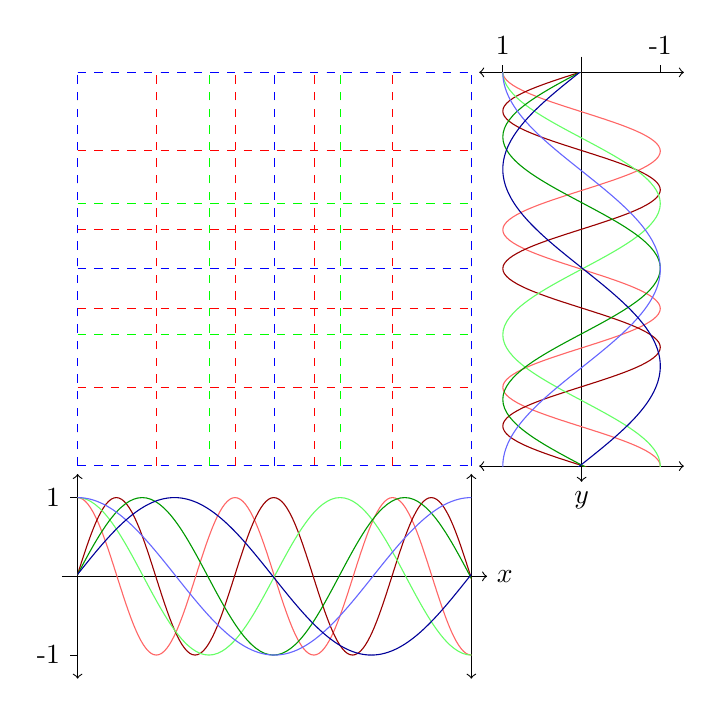
\begin{tikzpicture}[xscale=1, domain=0:4]
        \begin{scope}[yshift=40pt] % Draw grid lines
            \draw[help lines, color=red, dashed] (0,0) grid (5,5);
            \draw[help lines, color=green, dashed] (0,0) grid[step=5/3] (5,5);
            \draw[help lines, color=blue, dashed] (0,0) grid[step=5/2] (5,5);
        \end{scope}


    \begin{scope}[rotate around={-90:(6.4,0)}, yscale=-1]
        \draw[->] (-0.2,0) -- (5.2,0) node[below] {$y$};
        \draw[<->] (0,-1.3) -- (0,1.3);
        \draw (0,1) -- (-0.1,1) node[above] {1};
        \draw (0,-1) -- (-0.1,-1) node[above] {-1};
        \draw[<->] (5,-1.3) -- (5,1.3);
        \clip (0,-1.1) rectangle (5,1.1);
        \SinCos{red}{5}
        \SinCos{green}{3}
        \SinCos{blue}{2}
     \end{scope}

    \begin{scope}
        \draw[->] (-0.2,0) -- (5.2,0) node[right] {$x$};
        \draw[<->] (0,-1.3) -- (0,1.3);
        \draw (0,1) -- (-0.1,1) node[left] {1};
        \draw (0,-1) -- (-0.1,-1) node[left] {-1};
        \draw[<->] (5,-1.3) -- (5,1.3);

        \clip (0,-1.1) rectangle (5,1.1);

        \SinCos{red}{5}
        \SinCos{green}{3}
        \SinCos{blue}{2}
    \end{scope}

%        \begin{scope}[xscale=1/2]
%            \draw[color=red!60] (-1,0) sin (0,1) cos (1,0) sin (2,-1) cos (3,0) sin (4,1) cos (5,0) sin (6,-1) cos (7,0) sin (8,1) cos (9,0) sin (10,-1) cos (11,0) sin (12,1);
%%            \draw[color=red!60!black,xshift=-28pt] (0,0) sin (1,1) cos (2,0) sin(3,-1) cos(4,0) sin (5,1);
%
%            \draw[color=red!60!black, xshift=28pt] (-1,0) sin (0,1) cos (1,0) sin (2,-1) cos (3,0) sin (4,1) cos (5,0) sin (6,-1) cos (7,0) sin (8,1) cos (9,0) sin (10,-1) cos (11,0) sin (12,1);
%        \end{scope}
%        \begin{scope}[xscale=(5/3)/2]
%            \draw[color=green!60] (-1,0) sin (0,1) cos (1,0) sin (2,-1) cos (3,0) sin (4,1) cos (5,0) sin (6,-1) cos (7,0) sin (8,1) cos (9,0) sin (10,-1) cos (11,0) sin (12,1);
%            %            \draw[color=red!60!black,xshift=-28pt] (0,0) sin (1,1) cos (2,0) sin(3,-1) cos(4,0) sin (5,1);
%
%            \draw[color=green!60!black, xshift=28pt] (-1,0) sin (0,1) cos (1,0) sin (2,-1) cos (3,0) sin (4,1) cos (5,0) sin (6,-1) cos (7,0) sin (8,1) cos (9,0) sin (10,-1) cos (11,0) sin (12,1);
%        \end{scope}
    \end{tikzpicture}
\end{document}